\chapter{Przygotowania \emph{Know-how}}
\label{chap:know-how}
\section{Projektowanie REST API}
\label{sec:projektowanie-api}
Projektowanie i tworzenie API należy do podstawowych zadań programisty. Poprzez API odbywa się udostępnienie zasobów, jak również z nim związana jest ich ochrona. Zasobami najczęściej są dane, którymi klient może zarządzać w zakresie zdefiniowanym przez przypisane mu uprawnienia. Klientem może być strona internetowa służąca do wyświetlania i zarządzania danymi, a także inna aplikacja serwerowa korzystająca z tych danych.

Użycie API do dostarczania danych do aplikacji klienckiej pozwala rozdzielić logikę widoku po stronie klienta oraz logikę biznesową po stronie serwera. Zaletą tego rozwiązania jest uproszczenie implementacji i w dalszej perspektywie, ułatwienie utrzymywania tworzonego programu. Ponadto tak tworzone oprogramowanie jest bardziej elastyczne i łatwiej można je integrować z~innymi systemami. 

Stworzenie dobrego lub zmodyfikowanie już istniejącego API nie jest jednak zadaniem łatwym. Poza tym, że dodawanie funkcji filtrowania, sortowania czy łączenia danych z~różnych zasobów bywa po prostu nużące, to wymusza często konieczność tworzenia nowych punktów dostępu (ang.~\emph{endpoint}) do już istniejących zasobów lub modyfikowania tych już istniejących. Takie działanie niosą ze sobą ryzyko powstawania błędów. Problemem jest także budowanie adresu \texttt{URL} (ang.~\emph{Uniform Resource Locator}). Musi być on elastyczny i intuicyjny, aby można było pracować bez ciągłego wertowania dokumentacji. 

W dalszej części tego rozdziału zebrano zebrano dobre praktyki tworzenia API. Zwrócono też uwagę na zapoczątkowany przez Microsoft i zatwierdzony przez \texttt{ISO} (ang.~\emph{International Organization for Standardization}) protokół \texttt{OData} (ang.~\emph{Open Data Protocol}) i jego gotowe implementacje.

\subsection{Dobre praktyki tworzenia API} 
\label{subsec:api-dobre-praktyki}
Aby stworzyć czytelne i elastyczne REST API należy zastosować się do wielu zasad. Oczywiście nie są one obowiązkowe. Najczęściej jednak stosowanie się do nich ułatwia konsumowanie API i integrowanie go z innymi systemami. Jednym z koniecznych do szybkiej i bezproblemowej pracy z API kroków jest stworzenie i późniejsze aktualizowanie jego dokumentacji. Polecanym i nowoczesnym narzędziem służący do jej tworzenia jest \texttt{Swagger}. 

API projektujemy dla zasobów, które są rzeczownikami. Dlatego adres URL, a dokładniej jego ścieżka zasobów (ang.~\emph{resource path}) powinna być złożona z rzeczowników. Zalecane jest, aby używać liczby mnogiej rzeczownika, gdyż zazwyczaj zasób to zbiór przykładowo kont bankowych. Natomiast, aby wyrazić akcję, którą wykonuje się na zasobie należy użyć odpowiedniej metody \texttt{HTTP} (ang.~\emph{HTTP Verb}). W tabeli~\ref{tab:http-verb} widać wzorzec zastosowania metod HTTP~\cite{api-good-practises-1}.

\begin{table}
    \centering
    \caption{Użycie metod HTTP}
    \label{tab:http-verb}
    \begin{tcolorbox}[tab2,tabularx={X||Y|Y|Y|Y}]
    \texttt{Zasób}      & \texttt{GET}     & \texttt{POST}    & \texttt{PUT}      & \texttt{DELETE}   \\\hline\hline
    /bank-account   & Zwraca listę kont & Tworzy nowe konto &  Zbiorczo aktualizuje konta &  Usuwa wszystkie konta \\\hline
    /bank-account/1 & Zwraca określone konto & Metoda niedozwolona (405) &  Aktualizuje określone konto &  Usuwa określone konto \\\hline
    \end{tcolorbox}
\end{table} 

Kolejną ważną praktyką przy tworzeniu API jest zwracanie odpowiedniego kodu odpowiedzi HTTP (ang.~\emph{HTTP Status Code}), aby poinformować klienta o sposobie realizacji jego żądania. Żądanie może zakończone być sukcesem bądź niepowodzeniem. Jednak konieczne jest używanie więcej niż dwóch kodów odpowiedzi, aby dokładnie określić, co ten sukces lub niepowodzenie oznaczają. Dokument \texttt{RFC7231} opisuje, kiedy i jak używać konkretnych kodów odpowiedzi HTTP. Statusy HTTP dzielimy na pięć klas, które rozróżniane są po pierwszej cyfrze kodu odpowiedzi HTTP~\cite{rfc7231}.

\begin{itemize}
\item \texttt{1XX} -- Informacja -- Żądanie zostało odebrane, proces jest kontynuowany.  
\item \texttt{2XX} -- Sukces -- Żądanie zostało pomyślnie odebrane, zrozumiane i zaakceptowane. 
\item \texttt{3XX} -- Przekierowanie -- Konieczne jest podjęcie dalszych działań w celu zakończenia żądania.
\item \texttt{4XX} -- Błąd klienta -- Żądanie zawiera złą składnię lub nie może być zrealizowane.
\item \texttt{5XX} -- Błąd serwera -- Serwerowi nie udało zrealizować się poprawnego żądania.
\end{itemize}

W tabeli~\ref{tab:http-status} przedstawiono najczęściej używane w REST API statusy HTTP i ich znaczenie~\cite{api-good-practises-2, rfc7231}.  
Warto wspomnieć, że statusu \texttt{204} używa się najczęściej, gdy serwer nie zwraca w~ciele odpowiedzi żadnych danych. Sytuacją taką jest między innymi usuwanie zasobu.

\begin{table}
    \centering
    \caption{Kody odpowiedzi HTTP}
    \label{tab:http-status}
    \begin{tcolorbox}[tab2,tabularx={p{.30\linewidth}|Y}]
    \texttt{Kod HTTP}    & \texttt{Opis}   \\\hline\hline
    \texttt{200: OK}
        & Żądanie zakończone sukcesem. \\\hline
    \texttt{201: Created}
        & Stworzony został nowy zasób. \\\hline
    \texttt{204: No Content}
        & W ciele odpowiedzi nie ma żadnej dodatkowej treści.\\\hline
    \texttt{400: Bad Request}
        & Serwer nie może przetworzyć żądania z powodu błędu klienta.   \\\hline
    \texttt{401: Unauthorized}
        & Żądanie nie zostało przetworzone, ponieważ brakuje poprawnych danych uwierzytelniających dla docelowego zasobu. \\\hline
    \texttt{403: Forbidden}
        & Podane dane uwierzytelniające nie są wystarczające do autoryzacji żądania. \\\hline
    \texttt{404: Not Found}
        & Serwer źródłowy nie znalazł bieżącej reprezentacji zasobu docelowego lub nie chce ujawnić, że istnieje. \\\hline
    \texttt{500: Internal Server Error}
        & Serwer napotkał nieoczekiwany warunek, który uniemożliwił mu spełnienie żądania. \\\hline
    \end{tcolorbox}
\end{table}

Ważną zasadą dotyczącą API jest to, aby po stworzeniu nowego zasobu zwróciła jego reprezentację, na przykład w postaci \texttt{JSON} (ang.~\emph{JavaScript Object Notation}). Dotyczy to w szczególności metody \texttt{POST}. W przypadku powodzenia serwer powinien zwrócić w takim wypadku odpowiedź z kodem \texttt{201}, a także dodatkowy nagłówek z lokalizacją nowostworzonego zasobu (ang.~\emph{Location Header}). Dodatkowo rekomendowane jest, aby dane stworzonego obiektu lub obiektów zapakować w pole danych (ang.~\emph{data}) co~pokazano na listingu~\ref{list:response200}. 

{\belowcaptionskip=-10pt
\begin{lstlisting}[label=list:response200,
    caption=Przykład pomyślnej odpowiedzi serwera]
//200 OK
{
  "errors": [],
  "data": {
    "firstName": "Paweł",
    "lastName": "Żółaniecki",
    "age": 24
  }
}
\end{lstlisting}
}

Umieszczanie lokalizacji dostępnych zasobów wpisuję się w realizację koncepcji \texttt{HATEOAS} (ang.~\emph{Hypermedia As Transfer Engine Of Application State}). Pełna realizacja tej koncepcji zapewnia łatwą nawigację pomiędzy powiązanymi zasobami i przedstawia dostępne akcje na danym zasobie, poprzez umieszczanie w metadanych odpowiedzi linków URL do konkretnych akcji i zasobów.

W zależności od strategii biznesowej przyjętej w projekcie, gdy klient nie ma uprawnień do~zasobu, można zwrócić nie tylko kod \texttt{403}, ale także \texttt{404}, gdy serwer chce ukryć istnienie zasobu.

Dobrym zwyczajem jest umieszczanie w odpowiedzi z kodem \texttt{400} i \texttt{403} dokładniejszej informacji o przyczynie braku realizacji żądania. W podobny sposób powinno się informować klienta także o błędach. Częstą praktyką jest zwracanie w ciele odpowiedzi tabeli z listą błędów~\ref{list:response400}

{\belowcaptionskip=-10pt
\begin{lstlisting}[label=list:response400,
    caption=Odpowiedź serwera zawierająca opis błędu]
//400 Bad Request
{
  "errors": [
    {
      "status": 400,
      "details": "Invalid state. Valid state are 'draft', 'success' or 'failure'"
    }
  ]
}
\end{lstlisting}
}

Istotnym także jest, żeby nie tworzyć nowych adresów \texttt{URL} dla filtrowanego czy sortowanego zasobu. Lepszym podejściem jest przedstawić wyżej wymienione kryteria w ścieżce wyszukiwania adresu \texttt{URL} (ang.~\emph{query string}). W sekcji~\ref{subsec:odata} przedstawiony zostanie wybrany przez autora elastyczny protokół, określający strategię wyszukiwania i filtrowania zasobów za pomocą określonych parametrów ścieżki wyszukiwania adresu URL.

\subsection{Protokół OData}
\label{subsec:odata}

OData jest protokołem zbudowanym w oparciu o architekturę REST. Definiuje on nowe standardy i~praktyki budowania oraz konsumowania API. OData jest nie tylko standardem ISO, ale także \texttt{OASIS} (ang.~\emph{Organization for the Advancement of Structured Information Standards}). OData wykorzystywany jest w produktach firm takich jak: Microsoft, IBM, Telerik czy SAP. Standard definiowany przez OData sprawia, że konsumowanie API różnych dostawców opartych o ten protokół, staje się jednolite. Proces integracji nie wymaga przeznaczania dodatkowych nakładów pracy na naukę standardu danej organizacji~\cite{odata-why-use}.

OData umożliwia udostępnianie zasobów w postaci JSON, a także \texttt{XML} (ang.~\emph{Extensible Markup Language}). W obu wypadkach konwencje adresów URL, nagłówki itd.~pozostają takie same.
Biblioteki implementujące ten standard niejako zwalniają programistę z dbania o konwencje adresów URL, nagłówki żądań, metadane i kody odpowiedzi HTTP. 

OData oraz jego implementacje świetnie nadają się do szybkiego tworzenia REST API, a~na~pewno już tej jego części, która odpowiada za przetwarzanie zapytań (ang.~\emph{queries}). Zapytania są to operacje, które nie modyfikują stanu systemu, a jedynie zwracają dane, o które pyta klient. Zazwyczaj wykonywane są za pomocą metody HTTP GET. 

Charakterystyką zapytań jest to, że najczęściej klient nie potrzebuje wszystkich danych jakie są w systemie. Często na danych chce się wykonać projekcję, filtrowanie czy sortowanie. Nierzadko też potrzeba dokonać złączenia danych jednego zasobu z danymi innego zasobu. Filtrowanie i sortowanie to operacje, które często implementuje się w API z wykorzystaniem ścieżki wyszukiwania adresu URL. Operacja na listingu~\ref{list:odata-projekcja-sortowanie} pobiera imiona i wszystkich ludzi, posortowane malejąco według ich identyfikatora.

\begin{lstlisting}[label=list:odata-projekcja-sortowanie,
    caption=OData -- przykład projekcji i sortowania]
GET http://localhost:44300/api/odata/persons?$select=name, $orderby=id desc

{
  "odata.metadata":"http://localhost/odata/$metadata#Persons",
  "value":[
    {
      "name":"Paweł"
    },
    {
      "name":"Adaś"
    }
  ]
}
\end{lstlisting}

Podobne adresy URL można zaobserwować na innych stronach internetowych, które nie mają nic wspólnego z protokołem OData. Jednak prawdziwą zaletą OData jest umożliwienie agregacji danych kilku zasobów. To wszystko jest umożliwione programiście po napisaniu kilku dodatkowych linii kodu. Przykład agregacji widać na listingu~\ref{list:odata-agregacja}

\begin{lstlisting}[label=list:odata-agregacja,
    caption=OData -- przykład agregacji danych]
GET http://localhost/odata/persons?$expand=bank-accounts

{
  "odata.metadata":"http://localhost/odata/$metadata#Persons",
  "value":[
    {
      "bankAccounts":[
        {"id":1,"name":"Konto debetowe","balance":"15.49","ownerId":1},
        {"id":4,"name":"Lokata mobilna","balance":"10000.00","ownerId":1},
        {"id":5,"name":"Konto walutowe","balance":"00.00","ownerId":1}
      ],
      "id":1,
      "name":"Paweł"
    },
    {
      "bankAccounts":[
        {"id":3,"name":"Konto młodzieżowe","balance":"149.17","ownerId":2}
      ],
      "id":2,
      "name":"Adaś"
    }
  ]
}
\end{lstlisting}

Warto także zwrócić uwagę, że OData domyślnie dba za programistę o opakowanie informacji pobranych z API w pole danych, w tym wypadku \emph{values}. Tę dobrą praktykę wspomniano w punkcie~\ref{subsec:api-dobre-praktyki}. Obok interesujących nas danych znalazł się link do metadanych zasobu. Przy odpowiedniej konfiguracji i parametrach żądania pojawią się także parametry potrzebne m.in.~do~stronicowania.

Jak widać OData jest bardzo prosta w użyciu. Narzuca z góry dobrą konwencję adresów URL, a także zapewnia wiele wbudowanych generycznych funkcji, które znacząco przyśpieszają proces tworzenia oprogramowania.

\section{Użyte wzorce projektowe}
\label{sec:wzorce}

Jakość napisanego kodu jest bardzo ważna z punktu widzenia utrzymania i dalszego rozwoju systemu. Szczególnie istotna, a nawet niezbędna jest w dużych projektach, których proces rozwoju i utrzymania liczony jest w dekadach. Niezrozumiały i niejasny kod zwiększa znacząco ryzyko biznesowe i częstotliwość występowania błędów, nawet we wcześniej dobrze działających miejscach systemu.

Dla czystego kodu kluczowe jest luźne powiązanie (ang.~\emph{loose coupling}) komponentów czy klas. Termin ten oznacza podejście do tworzenia ich tak, aby zależności między nimi były jak najmniejsze. W skrócie wiedza elementów systemu o innych powinna być minimalna, a one same izolowane od siebie nawzajem oraz od zmian. Taka filozofia ma na celu zredukowanie ryzyka niezamierzonej zmiany działania pozostałych części systemu, a w konsekwencji doprowadzenia do krytycznego błędu. 

Idea luźnych powiązań jest ściśle związana z zasadami \texttt{SOLID}~\cite{clean-code}, a w szczególności pierwszej i ostatniej z nich. Pierwsza\label{ref:SRP}, czyli zasada pojedynczej odpowiedzialności (ang.~\emph{single responsibility principle}) określa, że każdy element systemu powinien mieć tylko jeden powód do zmiany. Jeden powód do zmiany przekłada się na jedną odpowiedzialność, a więc krótkie i zwięzłe funkcje czy klasy.

Ostatnia z~ww.~zasad -- zasada odwrócenia zależności (ang.~\emph{dependency inversion principle}) głosi, że klasy powinny być zależne od kontraktu, abstrakcji lub inaczej interfejsu, ale nigdy od konkretnych implementacji różnych serwisów. Stosowanie się do tych zasad zmniejsza powiązania, a co za tym idzie ułatwia rozszerzanie, modyfikowanie, a także testowanie kodu. Jednym słowem system staje się bardziej elastyczny.

\subsection{Mediator}
\label{subsec:mediator}

Mediator to wzorzec projektowy, którego głównym zadaniem jest utrzymywać w kodzie luźne powiązania i ograniczyć zależności między różnymi klasami. Mediator hermetyzuje komunikacje pomiędzy obiektami różnych klas udostępniając im interfejs, za pomocą którego się one komunikują. Tak więc celem mediatora jest usprawnienie czytania i utrzymania istniejącego kodu.

Popularną implementacją wzorca mediator jest biblioteka \texttt{MediatR}. Obudowuje ona proces komunikacji między klasami w abstrakcję żądań (ang.~\emph{request}) i zdarzeń (ang.~\emph{notification/event}). Obiekt używający mediatora może wysłać żądanie (ang.~\emph{send reqest}), które zostanie przechwycone przez inny obiekt tzw. ~\emph{handler}. Handler wykonuje zleconą operację i w zależności od implementacji może też zwrócić rezultat (ang.\emph{response})~\ref{fig:mediatR-Request}. Za przekazywanie tego żądania i odpowiedzi odpowiada mediator. Na rysunku~\ref{fig:mediatR-Request} widać przykład przepływu żądania wysłanego przez serwis.

\begin{figure}
	\centering
	\fbox{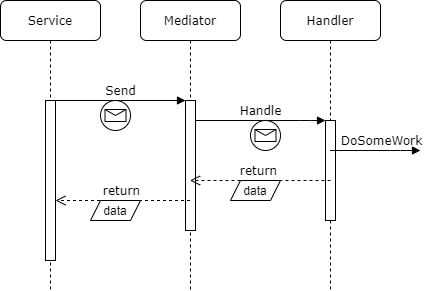
\includegraphics[width=.8\linewidth]{rys02/mediatR-Command.png}}
	\caption{Przykład wysłania żądania}
	\label{fig:mediatR-Request}
\end{figure}

Zdarzenia różnią się od żądań tym, że mogą być przechwytywane przez wiele handlerów. Z tego też powodu nie można zwrócić rezultatu zdarzenia. W pewnym sensie można w wielu scenariuszach odpowiedzieć na zdarzenie publikacją innego zdarzenia (ang.~\emph{publish event}). Jest to nowoczesna technika, która umożliwia asynchroniczne wywoływanie innych funkcji systemu, w szczególności w architekturze \texttt{mikroserwisów} (ang.~\emph{micorservices architecture}). Przykład publikacji zdarzeń można zaobserwować na rysunku~\ref{fig:mediatR-Event}.

\begin{figure}[h]
	\centering
	\fbox{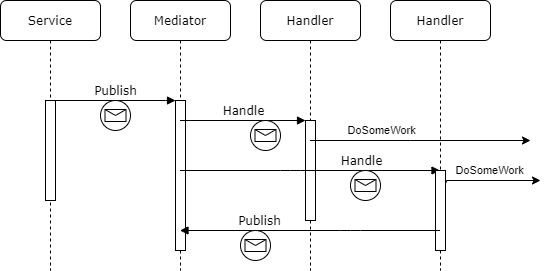
\includegraphics[width=.8\linewidth]{rys02/mediatR-Notification.png}}
	\caption{Przykład publikacji notyfikacji}
	\label{fig:mediatR-Event}
\end{figure}

\subsection{Podział odpowiedzialności czyli CQRS}
\label{subsec:cqrs}

Kolejnym wzorcem projektowym wartym uwagi w perspektywie tworzenia nowej aplikacji jest \texttt{CQRS} (ang.~\emph{Command Query Responsibility Segregation}). Pozwala on na użycie innego modelu do zapytań (ang.~\emph{queries}), czytających dane oraz do komend (ang.~\emph{command}), które modyfikują stan systemu. 

Na rysunku \ref{fig:cqrs-architecture} widać zarys architektury w przypadku bezstanowego API. Kierowane do API żądania HTTP GET przekazywane są do \emph{query} modelu, który czyta odpowiednie informację z bazy danych. Żądania POST przechwytuje \emph{command} model, posiadający skomplikowaną logikę biznesową, a następnie jeśli reguły biznesowe na to pozwalają, aktualizuje dane w magazynie danych. Wartym uwagi jest fakt, że oba modele mogą korzystać z innych połączeń do bazy danych, a więc model dla zapytań może nawet nie mieć uprawnień do zapisu w bazie danych. 

\begin{figure}[h]
	\centering
	\fbox{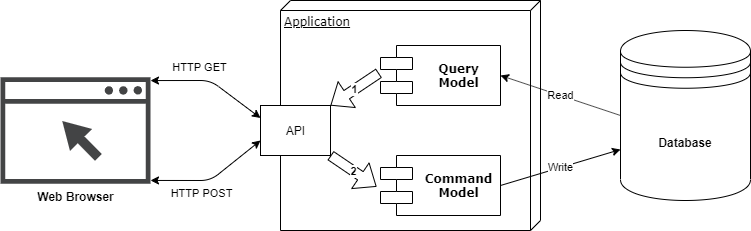
\includegraphics[width=.8\linewidth]{rys02/cqrs.png}}
	\caption{Architektura CQRS}
	\label{fig:cqrs-architecture}
\end{figure}

Gdy czytamy dane, często traktujemy aplikację serwerową jako opakowanie bazy danych -- swoisty kontener informacji~\cite{cqrs-fowler}. Najczęstszym, a także najważniejszym wymaganiem wobec zapytań jest ich wydajność. Natomiast podczas modyfikowania stanu systemu szybkość nie jest już krytycznym wymaganiem. Ważniejsze od niej są walidacja danych wejściowych, zgodność z regułami biznesowymi, obsługa wyjątków domenowych, a także atomowość operacji, tak aby pozostawić system w poprawnym stanie.

Segregacja komend i żądań pozwala dostosować kod źródłowy do specyficznych wymagań jakie się im stawia. Rozdziela ona także odpowiedzialność klas na wyższym poziomie systemu -- warstwie aplikacji. Dzięki temu powstają klasy wyspecjalizowane klasy warstwy aplikacji, które wykonują zapytanie, \texttt{albo} komendę. Mówi o tym także zasada pojedynczej odpowiedzialności\ref{chap:know-how}.

Ponadto CQRS idealnie komponuje się z systemem opartym o architekturę zdarzeń, którą oferuje np. biblioteka MediatR, opisana w punkcie~\ref{subsec:mediator}. CQRS dobrze działa także w architekturach opartych o \emph{event sourcing} czy \texttt{DDD} (ang.~\emph{Domain Driven Design}), a których autor szerzej nie opisze w tej pracy. 

\section{Autoryzacja OpenId Connect}
\label{sec:autoryzacja}